\documentclass{article}

\usepackage{a4wide}
\usepackage[utf8]{inputenc}
\usepackage[T1]{fontenc}
\usepackage[french]{babel}
\usepackage[babel=true]{csquotes} % guillemets français
\usepackage{graphicx}
\graphicspath{{Images/}}
\usepackage{color}
\usepackage{hyperref}
\hypersetup{colorlinks,linkcolor=,urlcolor=blue}

\usepackage{amsmath}
\usepackage{amssymb}


\title{Rapport TP de Programmation Concurrente}
\author{GASTELLIER Alison, L3 informatique}
\date{\today}

\begin{document}

\maketitle % pour écrire le titre


%% Le résumé:
\begin{abstract}
  Seront présentés dans ce rapport, les points importants et les diverses remarques sur les exercices 2.3 et 3.2 décrits ci-après.
\end{abstract}

\section{Introduction}
L'UE de programmation concurrente, intéressante quoique très courte, fut une très bonne occasion de jongler entre deux langages de programmation : le Python et le Java. Ces deux langages assez diamétralement opposés dans leur rédaction ont permis d'avoir une vue d'ensemble sur la rédaction de threads, c'est ce que l'on va voir dans ce rapport. J'ai choisi de travailler sur deux exercices différents.
Le premier exercice, que l'on va expliciter dans la première partie, traitera des files et sera intégralement rédigé en Python. Le deuxième exercice, rédigé en Java affichera des balles en mouvement à l'aide de threads.

%%%%%%%%%%%%%%%Exercice sur les files%%%%%%%%%%%%%%%
\section{Les files en Python}
\subsection{Explication de l'exercice}
Le programme que l'on avait à rédiger devait créer une file d'entiers (avec une capacité maximale) et ses différents threads, le producteur et les consommateurs, qui devront respectivement, alimenter la file et consommer les entiers de la file. Tout cela devra être présenté avec une interface sobre à l'aide du package TkInter de Python. 

\subsection{Parties de code}
J'ai séparé mon code en 3 parties distinctes. Un \textit{main}, une classe \textit{fenetre} qui lancera l'exécution des threads producteurs et consommateurs qui sont dans la dernière partie. 

\subsubsection{Partie 1 : Le \textit{main}}
Celui-ci comprends juste l'appel à la classe \textit{fenetre} et le mainloop pour afficher la petite interface.

\subsubsection{Partie 2 : La classe \textit{fenetre}}
La classe \textit{fenetre} comprends 2 fonctions : l'initialisation de la fenêtre (interface, boutons ...) et la fonction start qui va lancer 2 consommateurs et 2 producteurs en mode \textit{daemon}.
Pour la création de l'interface, je me suis aidée d'OpenClassroom \cite{OC_tkinter} et de la Doc de Python \cite{doc_python}.

\subsubsection{Partie 3 : Les classes \textit{FileAttente}, \textit{Producteur} et \textit{Consommateur} }

Ces trois classes si situent dans le fichier \textit{File\_Attente\_thread}.

La classe \textit{FileAttente} comporte 3 fonctions : l'initialisation, la méthode enfiler et défiler. J'ai choisi d'utiliser le module \textit{queue} de Python pour faire cet exercice.

\begin{enumerate}
\item La classe FileAttente

\begin{verbatim}
    def enfiler(self, nb):
        if(not self.q.full()):
            self.q.put(nb)
            self.liste.append(nb)


        self.labelFA.config(text = self.liste)


    def defiler(self):
        if(not self.q.empty()):
            self.liste.remove(self.liste[0])
            self.q.task_done()
        return self.q.get()
\end{verbatim}


Pour la méthode enfiler :
Si la file n'est pas pleine : ajouter un numéro à la file et à une liste locale qui m'a permis de me faciliter la tâche dans les affichages. En effet, les \textit{queue} en Python n'ont pas de méthode pour afficher la queue de manière simple. Cette liste sera donc affichée dans le label correspondant.

Pour la méthode defiler : 
Si la liste n'est pas vide, on peut enlever le premier élément de la liste (locale) et préciser que la tâche est terminée et retourner le premier élément de la queue.

\item La classe Producteur

Le producteur va produire des nombres aléatoires, l'enfiler (si possible) dans la queue puis afficher le nombre choisi dans l'interface. Quand le numéro a été intégré et affiché, le producteur attend un certain délai, qui permettra de décaler les différents threads producteur que l'on a crée.

\item La classe Consommateur

Le consommateur va défiler le premier numéro de la queue et ensuite afficher cet item dans le label et attendre pour décaler les différents threads.


\end{enumerate}

\subsection{Conclusion}

\begin{center}
  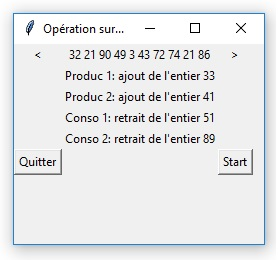
\includegraphics[scale=0.75]{Exercice23.png}
\end{center}

Ce programme très simple, repose principalement sur la rédaction des méthodes \textit{defiler} et \textit{enfiler}. Une fois ces fonctions écrites, l'écriture des threads principaux reste très simple. TKinter reste également simple d'utilisation à condition de prendre quand même le temps de trouver quelques exemples sur les forum ou autre.

%%%%%%%%%%%%%%%%Exercice sur les balles%%%%%%%%%%%%%%%
\section{Balles en mouvement}
\subsection{Explication de l'exercice}

Dans cet exercice, on devait écrire un programme qui permet d'afficher dans une fenêtre des balles en mouvement ( le nombre de balles étant fixe). L'utilisateur peut rajouter ou enlever des balles et ensuite démarrer ou arrêter l'animation. Lorsque deux balles se touchent, elles entrent en collision et devront être supprimées en ajoutant un point par collision. Combiné à tout ça, on a un petit timer qui indique le temps écoulé pendant le déplacement des balles.

\subsection{Parties de code}

Ici, j'ai séparé mon code en 4 parties. Un \textit{Maintag}, une classe \textit{Cercle}, une classe \textit{MaJFenetre} et finalement une classe \textit{Horloge} pour le timer. Voyons toutes ces classes détails.

\subsubsection{Partie 1 : Le \textit{main}}

Rien de particulier à dire sur cette partie qui ne sert uniquement qu'à lancer une instance de la classe fenêtre pour démarrer le programme.

\subsubsection{Partie 2 : \textit{Cercle}}

Pour faciliter la création de balles, j'ai rédigé la classe \textit{Cercle} avec comme attributs la position du centre du cercle et les constantes de déplacement. J'ai également crée des accesseurs à ces attributs pour me permettre de situer les balles et de gérer leurs déplacement. La méthode la plus importante ici est la méthode \textit{collision} :

\begin{verbatim}
	public boolean collision(int xpos, int ypos) {
		int a = x - xpos;
		int b = y - ypos;

		if ((a * a) + (b * b) <= 2 * r * 2 * r) {
			return true;
		}
		return false;
	}
\end{verbatim}

Cette méthode gère la collision entre deux balles distinctes et renverra un booléen pour indiquer si la collision a eu lieu ou non. Pour trouver la formule pour les collisions, je me suis aidée de OpenClassrooms \cite{OC_cercle} et des exercices de JAVA que j'ai eu avec Denis Payet en L2 \cite{DP_JAVA}.



\subsubsection{Partie 3 : \textit{Horloge}}

L'horloge est un thread lancé en même temps que le thread servant pour les balles que l'on décrira dans la prochaine section.
Cette classe possède deux méthodes. La méthode \textit{setpause} servira à modifier un booléen qui coupera le chrono ou lancera le chrono respectivement que les balles seront à l'arrêt ou en mouvement.
Pour ce qui est de la méthode \textit{run} : le thread va dormir une seconde, ajouter une seconde et l'afficher dans le label correspondant si et seulement si, l'utilisateur n'a pas mis une pause à l'animation.

\subsubsection{Partie 4  : \textit{MaJFenetre}}

Cette classe a été la partie la plus difficile du programme. Je ne m'étendrai pas ici sur le constructeur servant à afficher la fenêtre et placer les boutons. Je vais plutôt expliciter les méthodes \textit{movingball()} et \textit{actionPerformed()}.

\begin{enumerate}
\item movingball()

Cette méthode commence par créer un thread et  lier son runnable \textit{run()}. Run est divisé en trois parties. La première sert uniquement aux verouillages ou non des boutons si le maximum de balles que l'on a fixé a été atteint et pour vérifier que celui-ci ne soit pas inférieur à 0.
La deuxième partie gère le déplacement :

 \begin{verbatim}
	for (int i = 0; i < nb_actu_boules && liste_cercle[i] != null && !startstop; i++) {
						X = liste_cercle[i].getX();
						Y = liste_cercle[i].getY();

						if (X + 75 > 400 || X - 75 < 0) {
							liste_cercle[i].dx = -liste_cercle[i].dx;
						}
						if (Y + 75 > 575 || Y - 75 < 0) {
							liste_cercle[i].dy = -liste_cercle[i].dy;
						}

						X = X + liste_cercle[i].dx;
						Y = Y + liste_cercle[i].dy;

						liste_cercle[i].setXY(X, Y);
	
\end{verbatim}

Plus explicitement : pour chaque balles présentes dans la liste des balles (insérés dans un tableau \textit{liste\_cercle[]}) on va récuper la position du centre de la balle et vérifier qu'elle ne dépasse pas les bords de l'interface. Si c'est le cas, on inverse les direction et la balle partira dans l'autre sens. Une fois les composantes de mouvement changées, on fait appel à la méthode repaint() pour réafficher les balles. 
Ces actions ne vont être effectuées que si startstop vaut faux. Le booléen \textit{startstop} explicité dans la méthode ~\ref{item:start} actionPerformed.

A la fin du \textit{run()}, on va lancer le thread en lui-même qu'une seule fois : quand la méthode movingball() va être appelée, le thread va être lancé implicitement et va continuer de s'excuter.

La troisième partie gère les collisions :

\begin{verbatim}
				... suite directe du code juste en haut, on est toujours 
					dans la boucle avec l'incrément i ...
						for (int j = 0; j < nb_actu_boules; j++) {

							int xpos, ypos;

							if (liste_cercle[j] != null && liste_cercle[i] != null) {
								xpos = liste_cercle[j].getX();
								ypos = liste_cercle[j].getY();

								if (liste_cercle[i].collision(xpos, ypos) && i != j) {

									System.out.println("Boules " + i + " " + j + " entrées en colli");

									for (int k = i; k < nb_actu_boules - 1; k++) {
										liste_cercle[k] = liste_cercle[k + 1];
									}

									for (int l = j; l < nb_actu_boules - 1; l++) {
										liste_cercle[l] = liste_cercle[l + 1];
									}

									liste_cercle[nb_actu_boules - 1] = null;
									liste_cercle[nb_actu_boules - 2] = null;

									nb_actu_boules = nb_actu_boules - 2;

									System.out.println("Boules " + nb_actu_boules);

									// Modification du score total
									score++;
									score_tab.setText("Score : " + score);
\end{verbatim}

Cette partie est plus délicate. On compare chaque balles entre elles : s'il y a collision (grâce à la méthode écrite dans la classe Cercle), on décalle les cases du tableau de balles d'une jusqu'à la fin pour chacunes des balles impliquées dans cette dite collision ; dans le seul but de ranger les balles sans qu'il y ait de "trous" dans le tableau. Ensuite, on vide les deux dernières cases et on diminue le nombre total de boules de deux, on incrémente ensuite le score pour chaque collision.
J'ai décidé de laisser les "checks" des balles pour plus de clarté lors des tests.

\item actionPerformed
\label{item:start}

Cette méthode gère les actions effectuées sur les boutons de l'interface. Si l'utilisateur appuie sur le bouton "plus", il va pouvoir ajouter une balle sur l'écran :

\begin{verbatim}
x = (int) (Math.random() * 270 + 75);
			y = (int) (Math.random() * 370 + 75);

			// Vérification double spawn
			boolean check = true; // état de vérification
			boolean tour = false; // si une vérification a été faites ce tour-ci

			dance: while (check) {
				for (int j = 0; j < nb_actu_boules && liste_cercle[j] != null; j++) {
					if (liste_cercle[j].collision(x, y)) { // Si collision
						x = (int) (Math.random() * 270 + 75);
						y = (int) (Math.random() * 370 + 75);
						tour = true;
					}
				}
				if (!tour) {
					break dance; // on break si aucune vérification n'a été
									// faites
				}
				tour = false;
			}
\end{verbatim}

On attribut arbitrairement des coordonnées dans l'espace de l'interface et on vérifie que celles-ci ne sont pas déjà occupées par une autre balle. Ici, tant qu'une collision a été détectée entre 2 balles on continue à vérifier de nouveau pour toutes les balles présentes dans le tableau de base après avoir attribué de nouvelles coordonnées aléatoires. 
Si aucune collision n'a été détectée sur l'entièreté du tableau de balles, on peut casser le \textit{while} puis que les coordonnées déterminée ce tour-ci sont correctes.

\begin{verbatim}
// Ajout de la balle au pool de balles
			ball = new Cercle(x, y, 25, new Color(cred, cblue, cgreen));
			liste_cercle[nb_actu_boules] = ball;
			nb_actu_boules++;
\end{verbatim}

On va ensuite créer la balle correspondante et l'ajouter au tableau gobal de balles.

Dans le cas du "moins", la dernière balle du tableau gobal va être supprimée et la variable de qui indique le nombre de balles présentes sur l'interface va être actualisée.

Viens ensuite la dernière partie, si l'utilisateur appuie sur le bouton "start".

\begin{verbatim}
	if (startstop) {
				/*Quand le bouton Start est pressé*/
				h.setpause(false);
				movingball();
				startstop = false;
				start.setText("Stop");
				
			} else {
				/*Quand le bouton avec le label stop est pressé*/
				startstop = true;
				h.setpause(true);
				start.setText("Start");
			}
\end{verbatim}

Ici, quand le bouton start est pressé, on commence à faire tourner l'horloge (la pause est sur off) et on lance la fonction movingball() pour démarrer le thread et ainsi l'animation. Le booléen \textit{startstop} permet de savoir si l'on est en start ou en stop et on modifie l'affichage du texte sur le bouton en conséquence.
Si l'utilisateur appuie de nouveau sur le bouton, celui-ci aura le label "Stop", on rentre, ici, dans la partie else du if. On arrête l'horloge, le booléen \textit{startstop} passe à vrai (ce qui arrête le calcul des trajectoires des balles ainsi que le repaint()) et on modifie l'affichage du texte du bouton. 

\subsubsection{Conclusion}

\begin{center}
  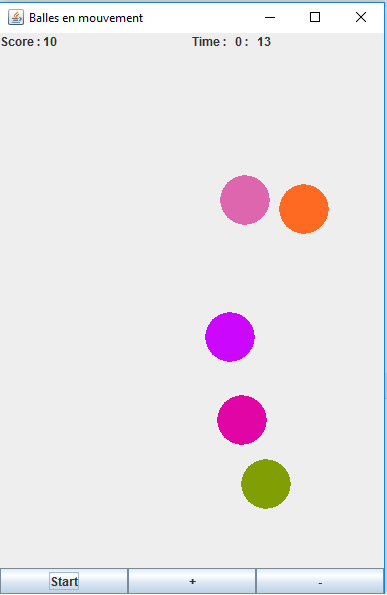
\includegraphics[scale=0.75]{Ballesmvt.png}
\end{center}

Cet exercice était beaucoup plus difficile que l'exercice des files. Je sais que mon programme peut être amélioré en soi et le principal problème que j'ai rencontré venait de la séparation du thread de l'UI. En effet, ici, l'UI gère beaucoup trop de choses ce qui ammène des erreurs dans l'utilisation de wait() et notifyall(). C'est pour cela que j'ai choisi l'utilisation des booléens pour arrêter les animations et le timer. 
\end{enumerate}

\section{Conclusion générale}

Le premier exercice était un exercice d'échauffement tandis que le deuxième demandait une maitrise du langage JAVA beaucoup plus poussée. Ils ont permis de couvrir une bonne partie de l'UE et nous permette d'approfondir nos connaissances dans le domaine de la programmation conccurente et des langages en eux-mêmes.



%%% La bibliographie:
\bibliographystyle{plain}
\bibliography{biblio}

\end{document}
